\documentclass{article}

  % if you need to pass options to natbib, use, e.g.:
  % \PassOptionsToPackage{numbers, compress}{natbib}
  % before loading nips_2018
  
  % ready for submission
  %\PassOptionsToPackage{numbers, compress}{natbib}
  \usepackage[final]{nips_2018}
  
  % to compile a preprint version, e.g., for submission to arXiv, add
  % add the [preprint] option:
  % \usepackage[preprint]{nips_2018}
  
  % to compile a camera-ready version, add the [final] option, e.g.:
  % \usepackage[final]{nips_2018}

  % to avoid loading the natbib package, add option nonatbib:
  % \usepackage[nonatbib]{nips_2018}
  
  \usepackage[utf8]{inputenc} % allow utf-8 input
  \usepackage[T1]{fontenc}    % use 8-bit T1 fonts
  \usepackage{hyperref}       % hyperlinks
  \usepackage{url}            % simple URL typesetting
  \usepackage{booktabs}       % professional-quality tables
  \usepackage{amsfonts}       % blackboard math symbols
  \usepackage{nicefrac}       % compact symbols for 1/2, etc.
  \usepackage{microtype}      % microtypography
  \usepackage{graphicx}
  \usepackage{caption}
  \usepackage{subcaption}
  \usepackage{multirow}
  % \usepackage{biblatex}
  % \addbibresource{final.bib}

  \title{Hate Speech Detection on Twitter}
  
  % The \author macro works with any number of authors. There are two
  % commands used to separate the names and addresses of multiple
  % authors: \And and \AND.
  %
  % Using \And between authors leaves it to LaTeX to determine where to
  % break the lines. Using \AND forces a line break at that point. So,
  % if LaTeX puts 3 of 4 authors names on the first line, and the last
  % on the second line, try using \AND instead of \And before the third
  % author name.
  
  \author{
    Jainul N.~Vaghasia\\
    Department of Computer Science\\
    University of Washington\\
    Seattle, WA 98105 \\
    \texttt{jnv3@cs.washington.edu}
    %% examples of more authors
    %% \And
    %% Coauthor \\
    %% Affiliation \\
    %% Address \\
    %% \texttt{email} \\
    %% \AND
    %% Coauthor \\
    %% Affiliation \\
    %% Address \\
    %% \texttt{email} \\
    %% \And
    %% Coauthor \\
    %% Affiliation \\
    %% Address \\
    %% \texttt{email} \\
    %% \And
    %% Coauthor \\
    %% Affiliation \\
    %% Address \\
    %% \texttt{email} \\
  }
  
  \begin{document}
  % \nipsfinalcopy is no longer used
  
  \maketitle

  \begin{abstract}
    We explore a neural network based method for classifying the presence of hate speech in a tweet.
    The network is based on word embeddings and average pooling, and produces state-of-the art results on
    offline model. The method when combined with resampling of subset of past training data performs well
    under severe class imbalance in online setting. With correct queue size, we obtain robust behavior against moderate concept drift in the stream as well.
  \end{abstract}
    
  \section{Introduction}
  Cyberbullying has become a rather common incident in that \cite{pew}
  found that, as of 2013, 73\% of people had witnessed harassment online, and a full
  40\% of people had experienced harassment directly. Such online harassment
  often includes posts with sexually violent language, threats, hate speech and degrading racist
  terms. Being able to identify cases of toxic tweets can therefore help in tackling this problem
  at its core. To this end, we frame the following binary classification problem:
  given a tweet, we wish to determine whether a tweet is offensive or not. There is no
  agreed upon definition of ``offensive'' owing to the ambiguities in human communication, but we
  use the following specific definition provided by \cite{hateoffensive}: ``language that is used to express hatred towards
  a targeted group or is intended to be derogatory, to humiliate, or to insult the members of the group.''
  
  We then approach this problem with two different perspectives. First, we handle the tweets in
  an offline manner in which tweets are provided
  in a batch beforehand. We optimize our model against class imbalance arising from the fact that offensive tweets are expected to be relatively fewer than non-offensive
  tweets. Second, we adapt our model for online learning where
  tweets arrive at different time steps such as when a reviewer flags a tweet as inappropriate. In doing so, we address the issue of class imbalance in the online setting while using minimal storage space.
   Furthermore, we address the phenomenon of concept drift which is defined as the variation of the underlying distribution of tweet classes with time.

  All code including backprop was written on basic libraries for instruction purposes and is available here: \url{https://github.com/JainulV/Hate-Detection-Twitter}.

  \section{Related Work}
  Many efforts have been made to classify hate speech using data scraped from online forums. \cite{waseem-hovy:2016:N16-2} and \cite{hateoffensive}
  applied logistic regression with engineered features such as n-grams, sentiment and tweet metadata on Sexism/Racism and HATE datasets respectively. \cite{founta2018unified} implemented two
  deep neural networks trained using transfer learning on tweet data and user metadata. \cite{2017OnTU} incorporate the use of simple word embeddings whose model we modify
  to use transformed word embeddings model (TWEM).

  In the realm of online learning, little work deals with class imbalance and concept drift each. Previous works of \cite{DBLP:journals/corr/abs-1804-02246} have modified the loss function to factor in weights of each class
  and perform a cost-sensitive online gradient descent. The problem is we need to know the class imbalance severity beforehand and since the cost remains static, it cannot deal with concept drift.
  Other strategies include oversampling and time decayed class size metric (\cite{Wang2015ResamplingBasedEM}) which either require abundant data or are static. For concept drift, a common strategy 
  is to use a sliding window over the data (\cite{Hoens2011LearningFS}). The drawback of this procedure is it does not handle class imbalance well. 

  This project seems to be the first attempt to address online learning problems of class imbalance and concept drift in hate speech detection on social networks.

  \section{Datasets}
  In this paper, we deal with two datasets to train and evaluate our classifier. First dataset
  is \cite{hateoffensive}'s publicly available HATE dataset compiled by searching for tweets on \url{www.Hatebase.org}.
  Tweets are binarized as ``hate speech'', or ``not''.
  The other dataset is \cite{Golbeck:2017:LLC:3091478.3091509}'s HAR harassment dataset, which identifies
  tweets as ``harassing'' or ``not''.\footnote{Available to researchers
  by emailing jgolbeck@umd.edu.} Retweets were removed from both datasets. Table~\ref{datasets-table}
  provides a numerical summary of both datasets. We also use 300 dimensional GloVe Common Crawl vector embeddings for translating words to vectors that are fed into our model
  (\citet{pennington2014glove}).

  \begin{table}
    \caption{Dataset Summary}
    \label{datasets-table}
    \centering
    \begin{tabular}{lll}
      \toprule
      %\multicolumn{2}{c}{Part}                   \\
      %\cmidrule(r){1-2}
      Name     & Labels and Counts     & Total \\
      \midrule
      \multirow{2}{*}{HATE} & Hate Speech \hspace{0.4cm} Not Hate Speech   &    \\
                             &  \hspace{0.2cm} \(1,430\) \hspace{2cm} \(23,353\) & $24,783$ \\
      \multirow{2}{*}{HAR} & Harassing \hspace{0.8cm} Not Harassing  &    \\
                             &  \hspace{0.2cm} $5,285$ \hspace{2cm} $15,075$ & $20,360$  \\
      \bottomrule
    \end{tabular}
  \end{table}

  \section{Methods}
  \subsection{Offline}
  Let us have \(\{(x^t, y^t)\}_{t=1}^n\) denote the training set where
  \(x^t\) is some tweet and \(y^t\) is the corresponding class label.
  We modify the TWEM method (\citet{kshirsagar2018predictive}) to use fewer parameters
  in exchange of minimal drop in accuracy. First, we create 300 dimenal embeddings for
  each word in a given tweet \(x^t\) of word length \(T\), so each word \(\{w_i\}_{i=1}^T\) in \(x^t\) is mapped to \(\{m_i\}_{i=1}^{T}\in \mathbb{R}^{300}\).
  We can preprocess the tweets before they are encoded with word embeddings but here we found that no significant increase in
  performance.
  Following this, we use average pooling operation on \(\{m_i\}_{i=1}^T\), which allows us to capture the overall
  context of the tweet. Denote the output from this operation as \(a\). This representation \(a\) is then fed
  into a 50 node 2-layer MLP followed by ReLU activation to allow for nonlinear representation learning.
  This is the penultimate layer which passes to a fully connected softmax layer with a class weighted cross entropy whose output is the probability
  distribution over the class labels.

  \subsection{Online}
  In order to adapt the above approach to online stream of tweets, we consider two queues of size \(L\)
  each, one holds the positive examples while the other holds the negative examples (\cite{Malialis2018QueueBasedRF}). Queue-based resampling stores the most recent example plus
  \(2L-1\) old ones. We will refer to the proposed algorithm as \(Queue_L\). The union of the two queues is then taken at each
  time step to form the new training set for the classifier. The cost function is given by
  \begin{equation} \label{eq:q}
      J=\frac{1}{|q^t|}\sum_{i=1}^{|q^t|} l(y_i, h(x_i)),
  \end{equation}
  where \(q^t\) is the union queue with \(|q^t|\leq 2L\) and \((x_i, y_i)\in q^t\); \(l(u_i, h(x_i))\) is any classification cost function. At each time step, the
  classifier weights are updated \textit{once} according to (\ref{eq:q}).  We direct the reader to the Appendix for the pseudocode and an illustrative diagram for Queue based Learning algorithm.

  The effectiveness of this approach can be attributed to the following highly intuitive reasoning. Having two queues keeps track of
  examples from both classes. It allows the classifier to ``remember'' old data from both classes, which can be seen as a form of oversampling to counteract the imbalance since the
  queue with less frequent examples will have same examples resampled more times than their counterparts. At the same time, we also note that since these queues are of
  fixed length \(L\), it allows the classifier to ``forget'' relatively old data and therefore act like a sliding window over the data stream. Fine-tuning the queue size for forgetfulness
  handles moderate concept drifts present in the stream.

  \section{Experiments and Results}
  \subsection{Offline}
  To train the neural network, we perform minimal preprocessing which includes tokenizing the data using Spacy and applying GloVe Common Crawl vector embeddings. 
  Training is performed using gradient descent with \(\ell_2\) regularization to reduce overfitting. The regularization parameter
  was chosen to be \(0.001\) by cross validation on 80--20 training-validation split.
  
  For comparing our model on HATE dataset, we borrow features engineered by \cite{hateoffensive} (which include part-of-speech ngrams, sentiment analysis, and Twitter specific features) and apply logistic regression. In addition, we use the statistics for
  Naive Bayes baseline and GRU model that uses metadata like popularity, network reciprocity and subscribed lists provided by \cite{founta2018unified}.
  For HAR dataset,
  \cite{kshirsagar2018predictive} offer performance for a baseline model trained using logistic regression with character ngrams, word unigrams and TF*IDF.

  The results are compiled in Table \ref{offline-res}. It is evident that our model requires relatively fewer preprocessing steps and depends only on tweet text, which eliminates dependence on
  retrieving features like social graphs, sentiment readability, etc. while performing better than these more complex approaches.

  \begin{table}
    \caption{Offline F1 Results}
    \label{offline-res}
    \centering
    \begin{tabular}{lll}
      \toprule
      %\multicolumn{2}{c}{Part}                   \\
      %\cmidrule(r){1-2}
      Method     & HATE     & HAR \\
      \midrule
      Logistic Regression (\cite{kshirsagar2018predictive}) & - & 0.68\\
      Logistic Regression (\cite{hateoffensive}) & 0.93 & -\\
      Naive Bayes & 0.82 & -\\
      GRU Text + Metadata (\cite{founta2018unified}) & 0.89 & -\\
      Ours & 0.94 & 0.70\\
      \bottomrule
    \end{tabular}
  \end{table}

  \subsection{Online}
  \begin{figure}
    \begin{center}
    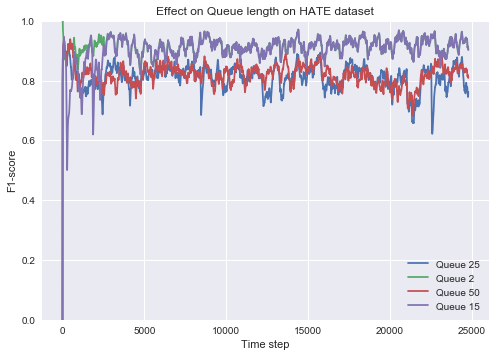
\includegraphics[width=2.25in]{Class_Imbalance_Result.png}
    \end{center}
    \caption{Prequential F1-Score against time step for different queue lengths}
    \label{fig:boat1}
  \end{figure}

  We begin by defining the prequential F1-score as our metric as suggested in \cite{Gama2012OnES}
  with a fading factor of \(\alpha=0.99\). At all time steps, we compute the prequential F1-score averaged over the most recent
  \(30\) runs.

  Having established the performance metrics, we inspect the performance on the problem of class imbalance. Our
  experiments show that without the Queue, the neural network only learns to predict majority class due to severe class imbalance in the online setting despite the use
  of weighted cross entropy. Henceforth, we focus on performance of \(Queue_L\) for \(L=\{2, 15, 25, 50\}\)  as shown in Figure \ref{fig:boat1}.
  \(Queue_2\) is the quickest to learn and performs the best
  followed by \(Queue_{15}\) which eventually matches the performance
  of \(Queue_2\) at about 3000th time step. Below, we shall experiment a trade-off for queue size that deals with concept drift. It is also seen that
  \(Queue_{25}\) and \(Queue_{50}\) lead to excessive oversampling which forces the classifier to ``remember'' old data for a long time, thereby affecting
  the decision boundary. Consequently, they are not able to perform as good as the former algorithms.

  \begin{figure}
    \centering
    \begin{subfigure}{.5\textwidth}
      \centering
      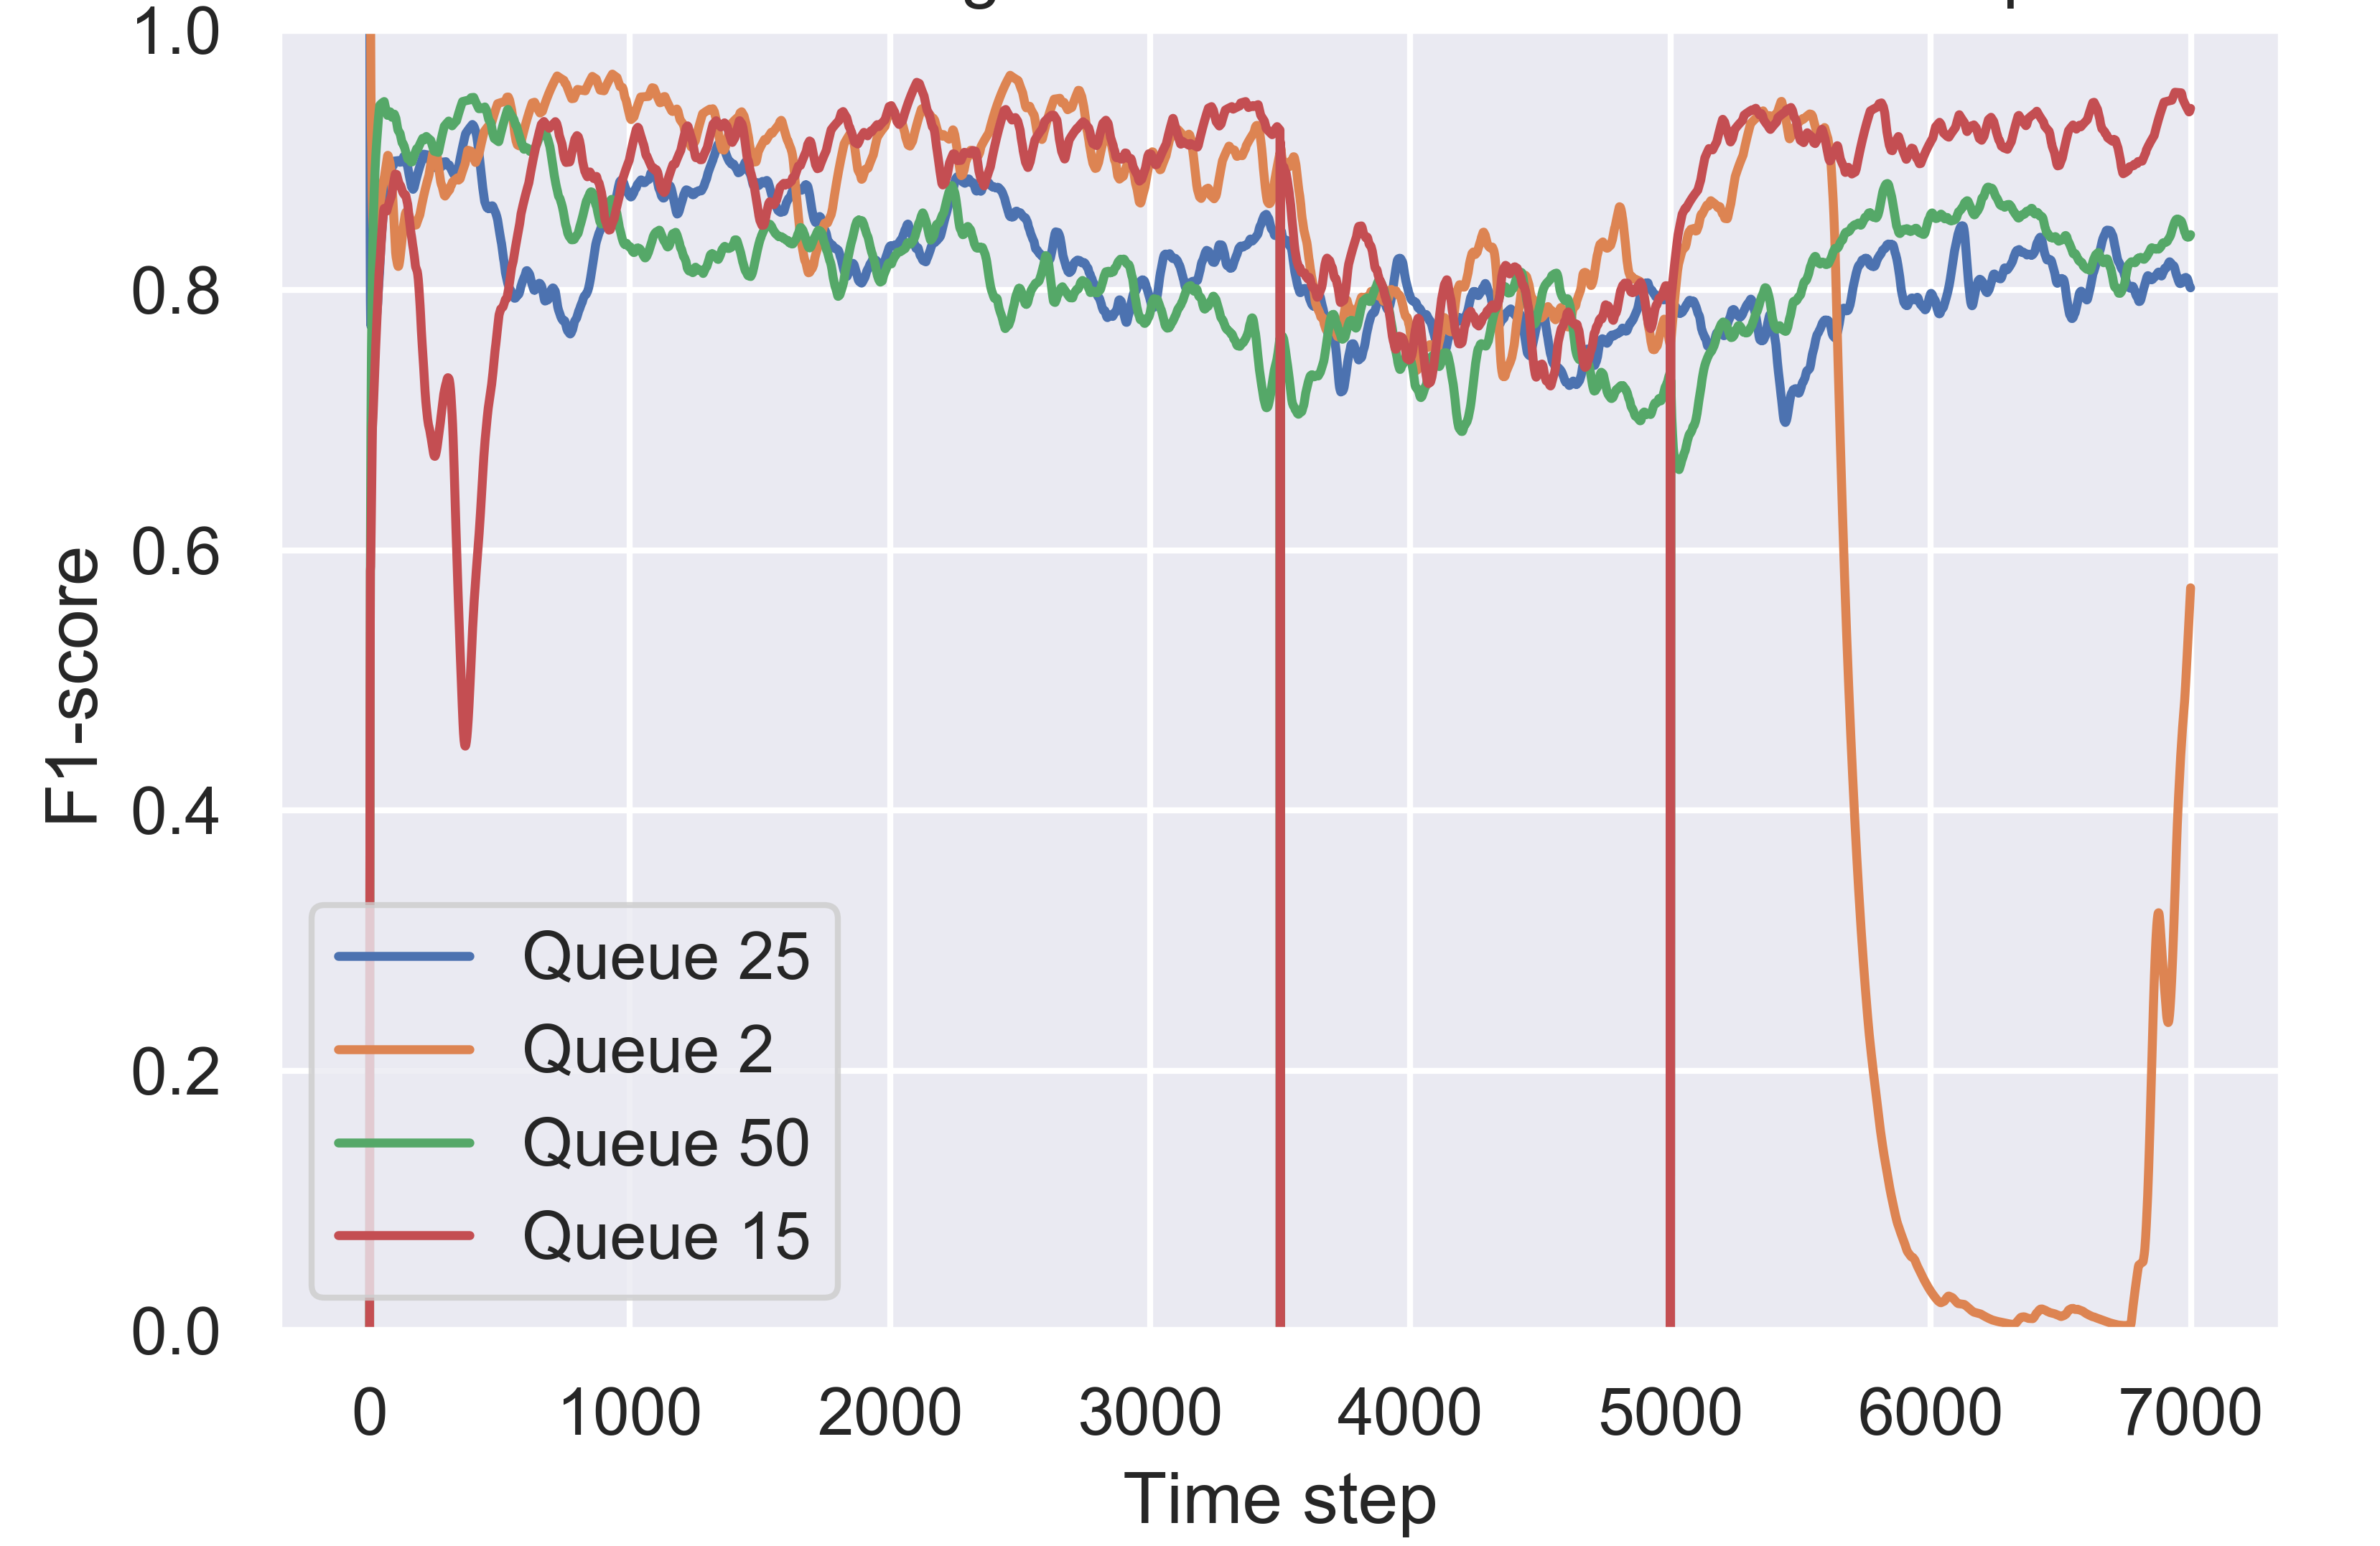
\includegraphics[width=2.5in]{concept_drift_more.png}
      \subcaption{}
      \label{fig:sub1}
    \end{subfigure}%
    \begin{subfigure}{.5\textwidth}
      \centering
      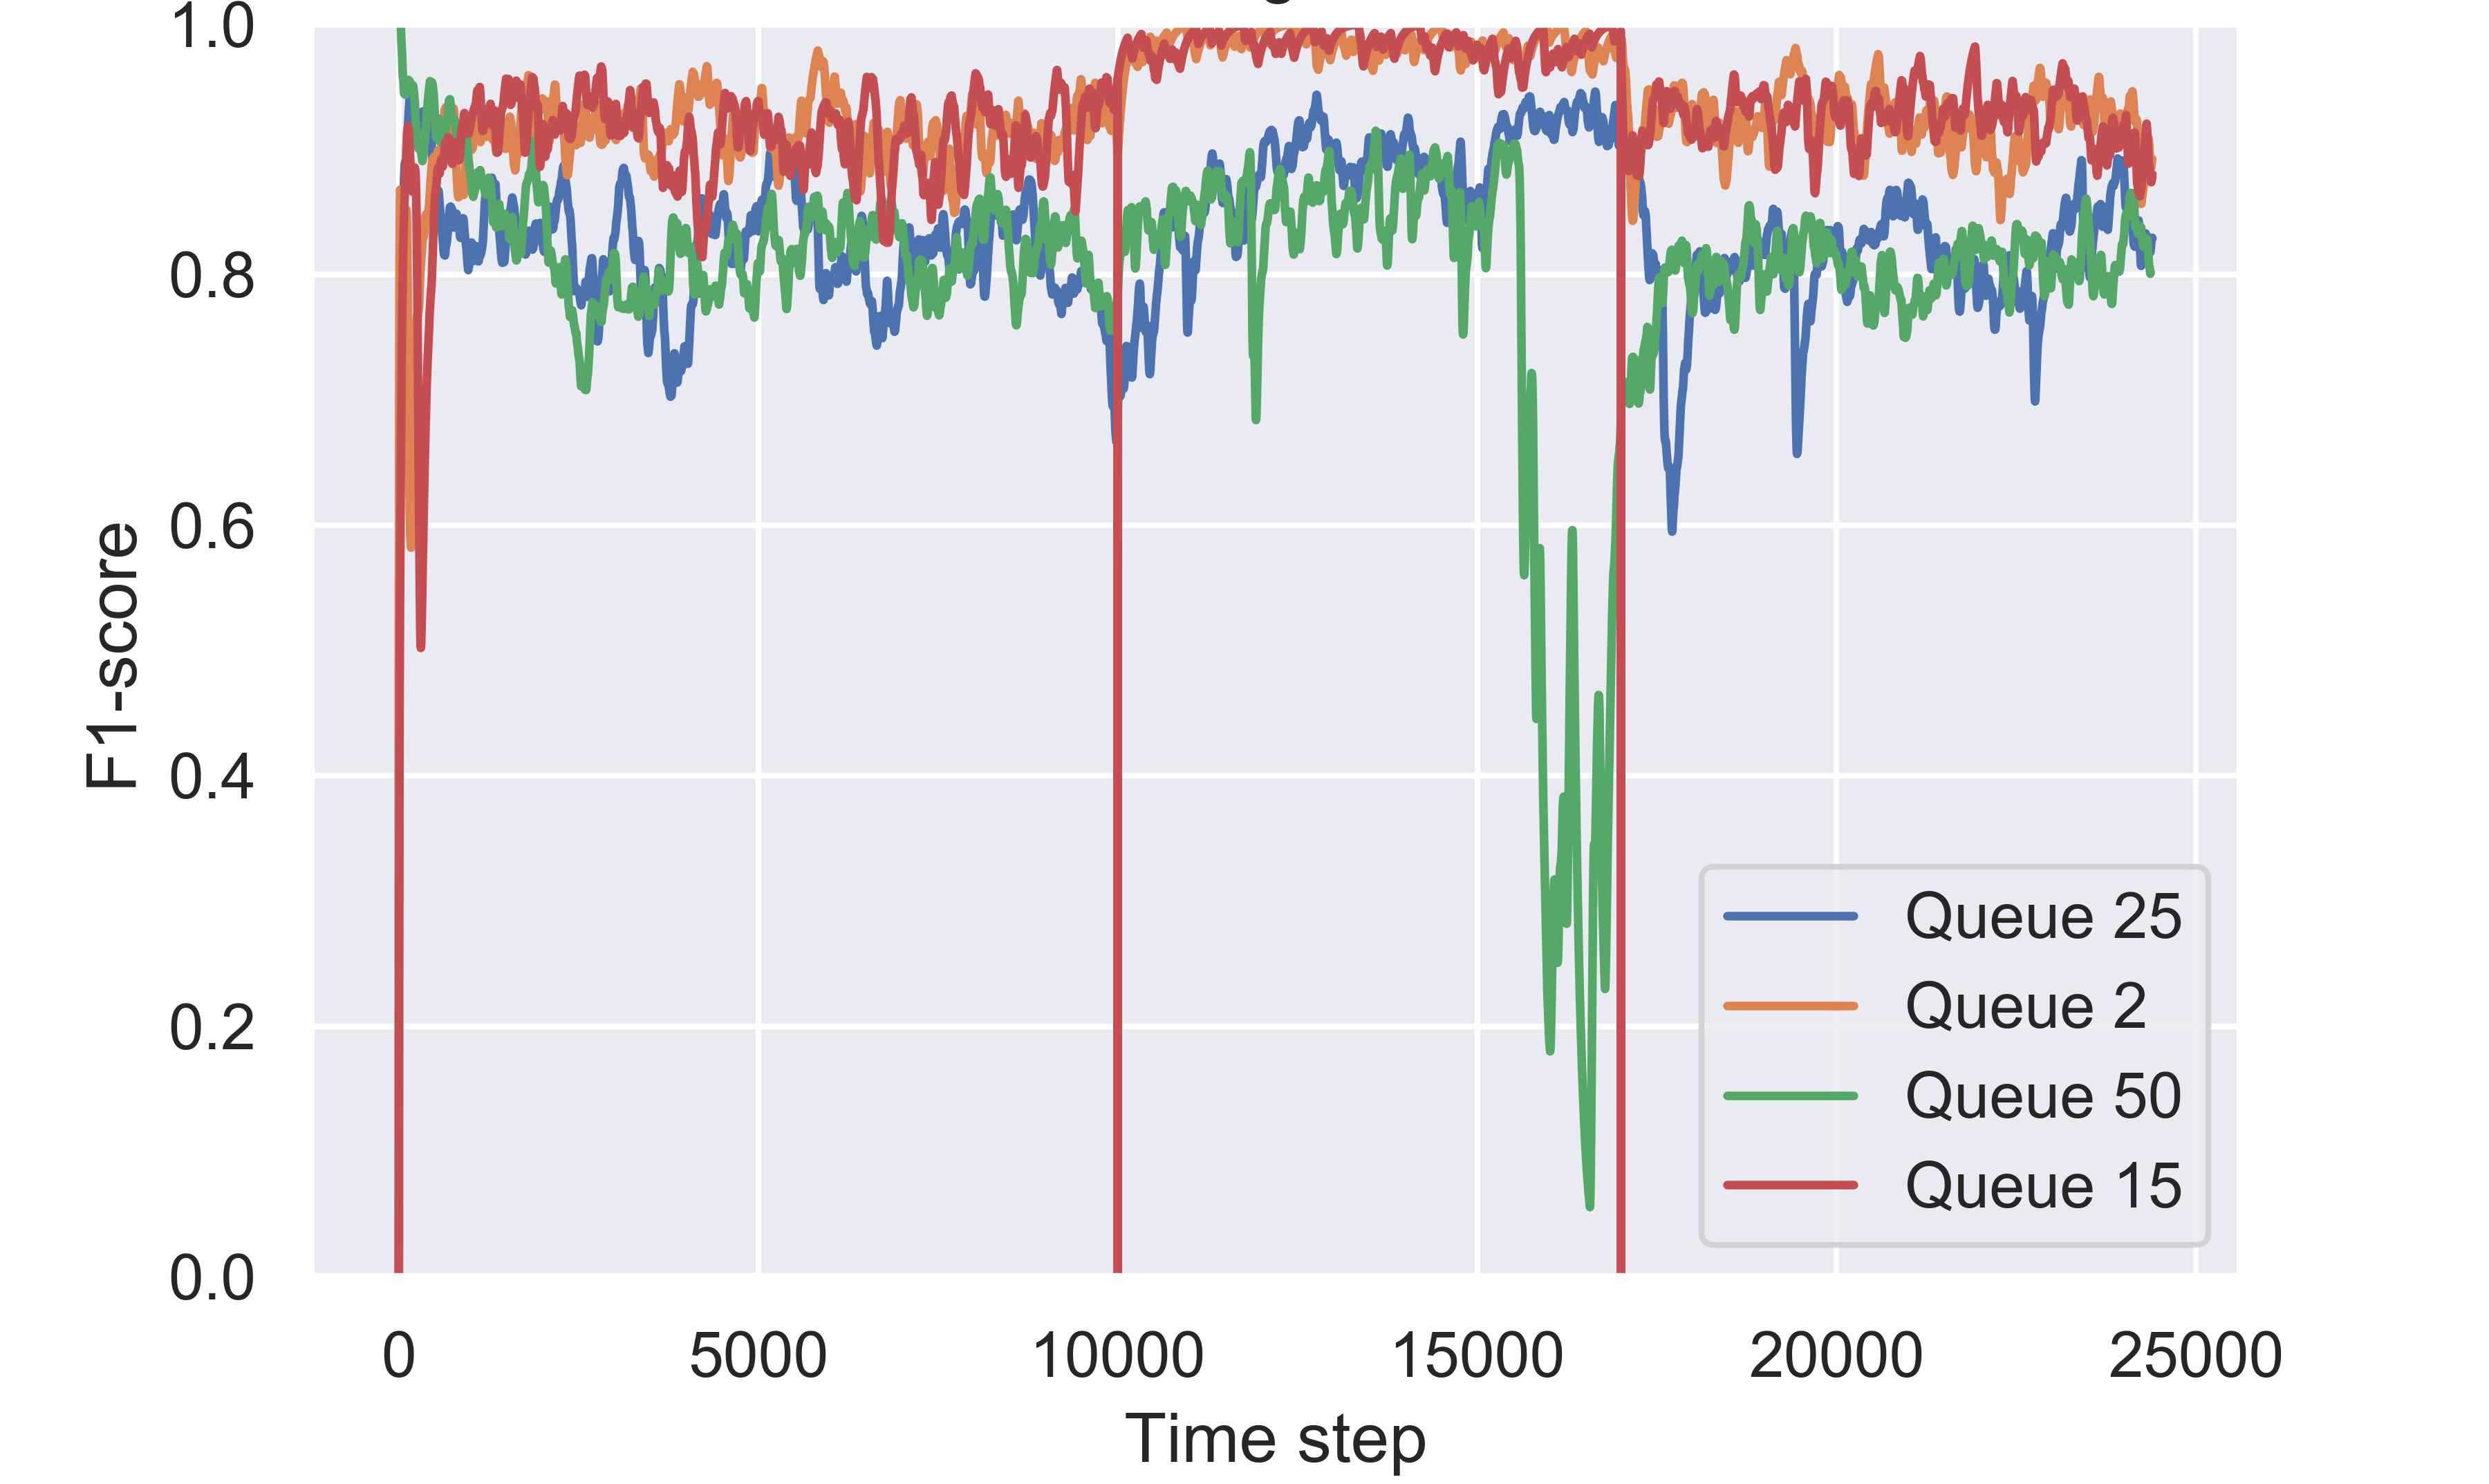
\includegraphics[width=2.5in]{concept_drift.png}
      \vspace{0.01pt}
      \subcaption{}
      \label{fig:sub2}
    \end{subfigure}
    \caption{Performance under changing probability distribution. (\ref{fig:sub1}) Probability of positive class increases from 0.05 to 0.15 at time step 3500 and
    back to 0.05 at 5000th time step. (\ref{fig:sub2}) Probability of positive class decreases from 0.05 to 0.01 at time step 10000 and
    back to 0.05 at 17000.}
    \label{fig:test}
  \end{figure}

  Next, we experiment with concept drift where we induce a change in the sampling probabilities for the positive (offensive)
  class at different time steps. These drifts are mild in the sense that the majority class label does not change as a result of the drift.
  We note that to preserve the performance metric from being affected by the drift, we reset it to 0 at the drift point.

  In the first experiment, we increase the probability of positive class from 0.05 to 0.15 after the 3500th tweet and then drop it back to 0.05
  at 5000th time step. The results are depicted in Figure (\ref{fig:sub1}). Contrary to the competitive performance of \(Queue_2\) under class imbalance,
  here we see that it takes longer for \(Queue_2\) to recover from drift due to very few stored samples while the drift flushes these samples. 
  \(Queue_{25}\) and \(Queue_{50}\) still suffer from excessive oversampling but are able to recover. \(Queue_{15}\) balances the oversampling and recovery the best.
  
  Changing the direction of the drift, in the next experiment, we decrease the probability of positive to 0.01 at 10000th tweet and bring it back up to
  0.05 at 17000th tweet as shown in Figure (\ref{fig:sub2}). In this case, \(Queue_2\) and \(Queue_{15}\) behave with almost the same performance.
  \(Queue_{25}\) does not quite beat its lower size counterparts but still recovers. \(Queue_{50}\) has too many samples to affect its training when the
  class imbalance is in severe phase at 0.01 (cf. performance of \(Queue_2\) in the previous case).


  \section{Conclusion}
  We explored an offline model that requires a minimal amount of feature engineering and outperforms its counterparts on the task of classifying a tweet as
  offensive or otherwise. In online setting, we show that the queue based resampling heuristic is able to handle class imbalance and abrupt concept drifts.
  Future work includes evaluating the effectiveness under other types of drifts (eg. gradual) and the amount of tuning required for queue length. We would also like to see explore methods
  to deal with noisy labels. Such a method would greatly reduce the amount of tweets to be reviewed by hands.
  

  \newpage
  \bibliographystyle{plainnat}
  \bibliography{final}

  \newpage
  \section*{Appendix}
  Included in this appendix are the queue learning algorithm and an illustrative diagram on how the process works (\cite{Malialis2018QueueBasedRF}).
  \begin{center}
  \includegraphics[width=4in]{Queue.png}
  \end{center}
  \includegraphics[width=\linewidth]{algo.png}
  \end{document}